\documentclass[a4paper]{article}
\usepackage{listings}
\usepackage{verbatim}
\usepackage{graphicx}
\usepackage{amsmath}
%% Language and font encodings
\usepackage[english]{babel}
\usepackage[utf8x]{inputenc}
\usepackage[T1]{fontenc}

%% Sets page size and margins
\usepackage[a4paper,top=3cm,bottom=2cm,left=3cm,right=3cm,marginparwidth=1.75cm]{geometry}

%% Useful packages
\usepackage{amsmath}
\usepackage{graphicx}
\usepackage[colorinlistoftodos]{todonotes}
\usepackage[colorlinks=true, allcolors=blue]{hyperref}

\begin{document}
\begin{titlepage}
	\raggedleft
	\rule{1pt}{\textheight} 
	\hspace{0.05\textwidth} 
	\parbox[b]{0.75\textwidth}{		
		{\LARGE\bfseries EE - 2703 Applied Programming Lab \\[0.5\baselineskip]  ~\huge Assignment -5}\\[2\baselineskip] 
		{\large\textit{Laplace Equation}}\\[4\baselineskip] 
		{\Large\textbf{Mohammed Khandwawala}}
        \large EE16B117
		\vspace{0.5\textheight}  
	}

\end{titlepage}


\tableofcontents


\section{Introduction}



We wish to solve for the currents in a resistor.
A wire is soldered to the middle of a copper plate and its voltage is held at 1 Volt.  One side of the plate is
grounded, while the remaining are floating. The plate is 1 cm by 1 cm in size.
As a result,  current flows.   The current at each
point can be described by a “current density”. This
current density is related to the local Electric Field by the conductivity:
$$ \vec{j} = \sigma \vec{E} $$
Now the Electric field is the gradient of the potential,
$$ \vec{E} = -\nabla \phi $$
and continuity of charge yields
Combining these equations we obtain
$$ \nabla \vec{j} = -\frac{d\rho}{dt}$$
Assuming that our resistor contains a material of constant conductivity, the equation becomes
$$ \nabla . (-\sigma \nabla \phi) = -\frac{d\rho}{dt} $$
For DC currents, the right side is zero, and we obtain
$$  \nabla^{2} \phi = 0 $$

\section{Defining the parameters}

Defining grid size (the size of the resistor) , the radius of the conductor and the number of iterations to run for converging the result.
\begin{lstlisting}[language=Python]
# declaring the constants 
Nx = 25	# size of the grid
Ny = 25
radius = 8; # radius of the wire
Niter = 1500;

\end{lstlisting}


\section{Allocating potential array and initialization}
An array phi is crated with initial value 0 of dimensions Nx by Ny. It will look like
\begin{gather}
 \begin{bmatrix} 0 & 0 & 0 & ... & 0 & 0 \\  0 & 0 & 0 & ... & 0 & 0 \\ ... & ... & ...& ...& ... \\0 & 0 & 0 & ... & 0 & 0 \end{bmatrix}
 \end{gather}
Since we want the origin at the center of the grid.  Create two axis from $\frac{-Nx}{2}$ to $\frac{Nx}{2}$ and $\frac{-Ny}{2}$ to $\frac{Ny}{2}$
Using python function meshgrid we can get coordinates for the above to axis array.
using the condition that potential inside the conductor is uniform and constant so phi inside the circle should be 1 at all point.
X$^{2}$ + Y$^{2}$ < 8*8 .
Storing these points and using np.where command to make potential 1 in phi grid.
\begin{lstlisting}[language=Python]
# creating vectors x,y for 2-D coordinates
print -Nx/(2*25.0),Ny/(2*25.0)
x = np.linspace(-Nx/(2*25.0),Ny/(2*25.0),25)
y = np.linspace(-Nx/(2*25.0),Ny/(2*25.0),25)

#Y,X coordinates of the grid which we will create
Y,X = np.meshgrid(x,y)

#selecting coordinates inside the circular conductor
ii = np.where(X*X+Y*Y<=(0.35)**2)

#creating grid and marking potential inside the circle 1
phi = np.zeros((Nx,Ny))
phi[ii] = 1

\end{lstlisting}
\subsection{Plotting Contour Plot}
\begin{lstlisting}[language=Python]
plt.contour(Y,X,phi)
plt.plot(x[ii[0]],y[ii[1]],'ro')
plt.show()
\end{lstlisting}
\begin{figure}
\caption{Contour plot for potential of conductor when no current is flowing in the resistor}
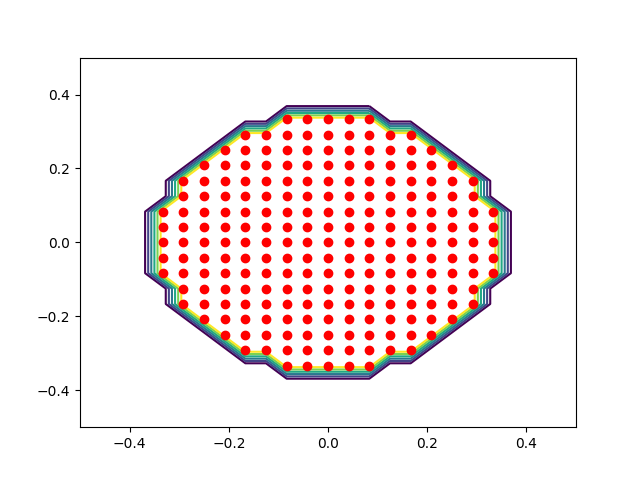
\includegraphics{Figure_1-2.png}
\end{figure}
\section{Perform the iterations}
Now we need to iteratively update potentials for that we need to store old phi matrix , update value , assert boundary conditions and compute error (change).
For storing we need to use python copy as normals equals operator does not generate a new phi it will just give it one more reference.
Laplace’s equation is easily transformed into a difference equation.   The equation can be written out in
Cartesian coordinates
$$$$
Assuming $\phi$ is available at points (x$_{i}$,y$_{i}$)
we can write
$$ \frac{d\phi}{dx}_{(x_{i},y_{i})} = \frac{\phi(x_{i+1/2},y_{j})\phi(x_{i-1/2},y_{j})}{\Delta x} $$
and
$$ \frac{d^{2}\phi}{dx^{2}}_{(x_{i},y_{i})} = \frac{\phi(x_{i+1},y_{j})-2\phi(x_{i},y_{j})+\phi(x_{i-1},y_{j})}{\Delta x} $$
Combining this with the corresponding equation for the y derivatives, we obtain
$$\phi_{i,j} = \frac{\phi_{i-1,j}+\phi_{i,j-1}+\phi_{i,j+1}+\phi_{i+1,j}}{4}$$
Thus, if the solution holds, the potential at any point should be the average of its neighbors.

Using the result we will update phi matrix by taking the average of the neighbors.

For Boundary conditions we know that the lower edge is grounded so it is at constant 0 potential.
the other three sides we know the current can ot flow outwards so we will make the gradient of potential along each side 0. That is by equating it to value of potential one column before. 

For measuring error we will take the maximum of absolute difference between old and new phi matrix.
\begin{lstlisting}[language=Python]
errors = np.zeros(Niter)
for k in range(Niter):
	oldphi = phi.copy()
	phi[1:-1,1:-1] = 0.25*(phi[1:-1,0:-2]+phi[1:-1,2:]+phi[0:-2,1:-1]+phi[2:,1:-1]) #updating potential as mean of its neighbors
	phi[1:-1,0] = phi[1:-1,1] # Boundary Conditions
	phi[1:-1,-1] = phi[1:-1,-2]
	phi[0,:] = phi[1,:]
	phi[-1,:] = 0 # lower plate potential is 0
	phi[ii] = 1.0		
	errors[k] = (abs(phi-oldphi)).max(); #error measurment 
\end{lstlisting}

\subsection{Surface Plot of Potential}
Plotting the 3-D plot representing potential on each point of the surface.
\begin{lstlisting}[language=Python]
#3-D surface plot of potential
fig1 = plt.figure(1)
ax = p3.Axes3D(fig1)
plt.title('The 3-D surface plot of potential')
surf = ax.plot_surface(-Y,-X,phi.T,rstride = 1,cstride = 1, cmap = plt.cm.jet)
plt.show()

\end{lstlisting}
\begin{figure}
\caption{3-D plot representing voltage at different points}
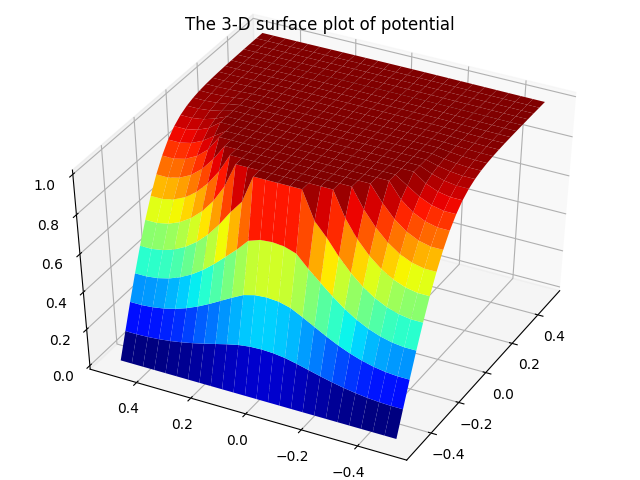
\includegraphics{Figure_1-3.png}
\end{figure}
\subsection{Contour plot of potential}
\begin{lstlisting}[language=Python]

#contour plot of potentials
plt.contour(-X,-Y,phi)
plt.plot(y[ii[0]],x[ii[1]],'ro')
plt.show()
\end{lstlisting}
\begin{figure}
\caption{}
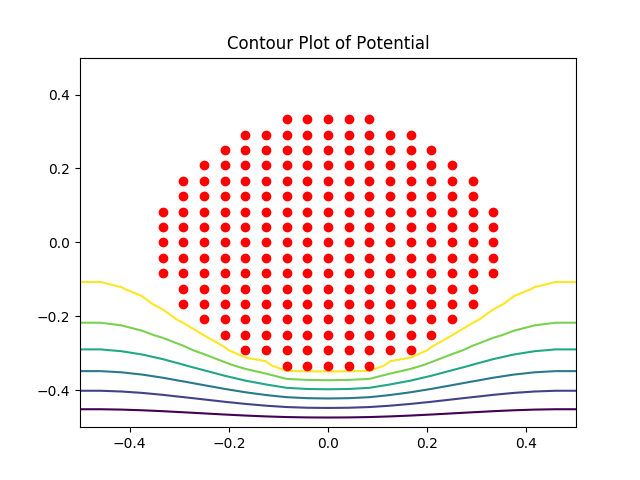
\includegraphics{Figure_1-4.png}
\end{figure}

\subsection{Vector Plot of Current}
Now to obtaint the current we need to calculate the gradient of the potential.
$$ j_{x} = \frac{-d\phi}{dx}$$
$$ j_{y} = \frac{-d\phi}{dy}$$
This numerically translates to
$$ j_{x,ij} =  \frac{1}{2}(\phi_{i,j-1} - \phi_{i,j+1})$$
$$ j_{y,ij} =  \frac{1}{2}(\phi_{i-1,j} - \phi_{i+1,j})$$

vector plots can plotted using quiver function.
\begin{lstlisting}[language=Python]

#vector plot of the electric field
Jx = np.zeros((Nx,Ny))
Jy = np.zeros((Nx,Ny))
Jx[1:-1,1:-1] = 0.5*(phi[1:-1,0:-2]-phi[1:-1,2:])
Jy[1:-1,1:-1] = 0.5*(phi[0:-2,1:-1]-phi[2:,1:-1])
plt.quiver(y,x,-Jx[::-1,:],-Jy[::-1,:])
plt.plot(y[ii[0]],x[ii[1]],'ro')
plt.show()
\end{lstlisting}
\begin{figure}
\caption{}
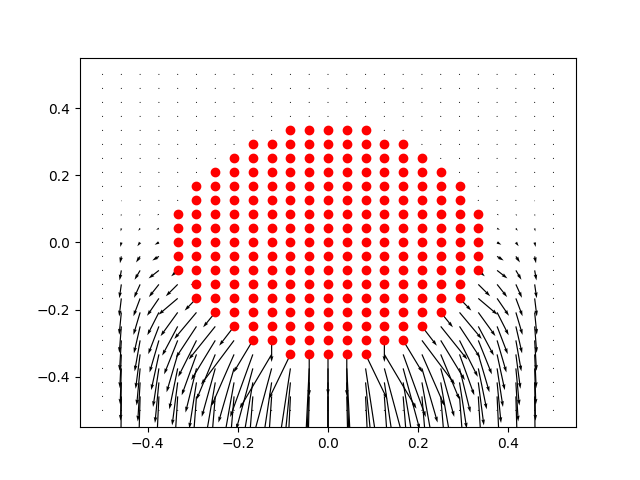
\includegraphics{Figure_1-5.png}
\end{figure}
\subsection{Explanation of the graph}
As seen from contour plot of potential ,current obtained here is perpendicular to equipotential. And the current negligible in the other half because the current flow through the path of least resistance . The path between the 1V conductor and ground in through lower half of the plate and thus no current flows through the upper half.
\section{Error Analysis}

\begin{lstlisting}[language=Python]
plt.semilogy(errors)
plt.label("Semi-log plot of Error vs iterations")
plt.show()
\end{lstlisting}
\begin{figure}
\caption{}
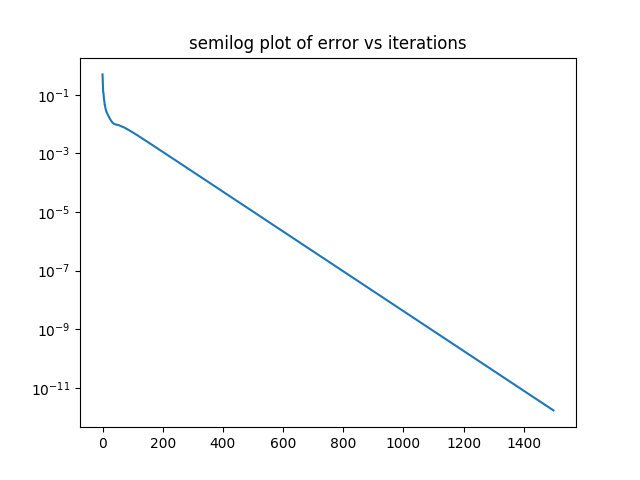
\includegraphics{Figure_1-6.png}
\end{figure}
This semilog plot of error shows straight line with negative slope. Error in this case falls as Ae$^{B*k}$ whrere k is number of iterations and A,B are constants. So error can can be written as
$$ log(error) = log(A) + B*k $$
With the error obtained we can fit it to the straight line to obtain constants A and B.
We sample error at 50 points and then obtain a fit . fitting complete data. In second cane we will take error only after 500 iterations.
\begin{lstlisting}[language=Python]
#fitting error model
#creating matrix of coeff 
A = np.zeros((Niter/50,2))
A[:,0] = 1
A[:,1] = np.log(np.arange(1,Niter+1,50))
#finding unknown variable to fit error
fit_1 = linalg.lstsq(A,np.log(errors50))[0]

#fitting error model excluding first 500 points
A = np.zeros(((Niter-500)/50,2))
A[:,0] = 1
A[:,1] = np.log(np.arange(501,Niter+1,50))
fit_2 = linalg.lstsq(A,np.log(errors50[10:]))[0]

#printing coeffs obtained by both the model
print fit_1
print fit_2

\end{lstlisting}

Now we will plot the above two cases along with actual error plot and see which one data gave a better fit.
\begin{figure}
\caption{}
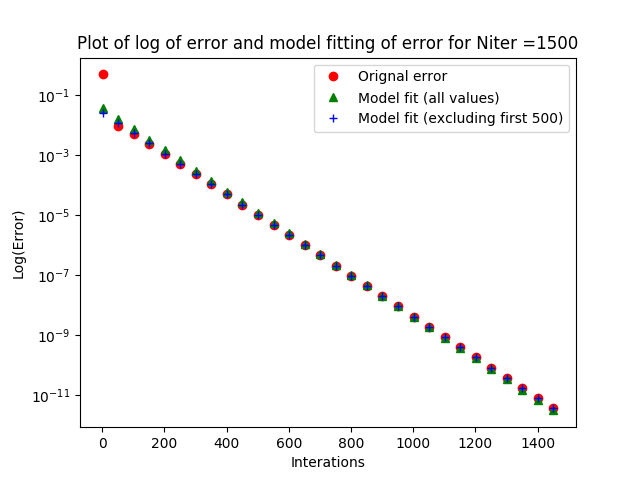
\includegraphics{Figure_1-7.png}
\caption{}
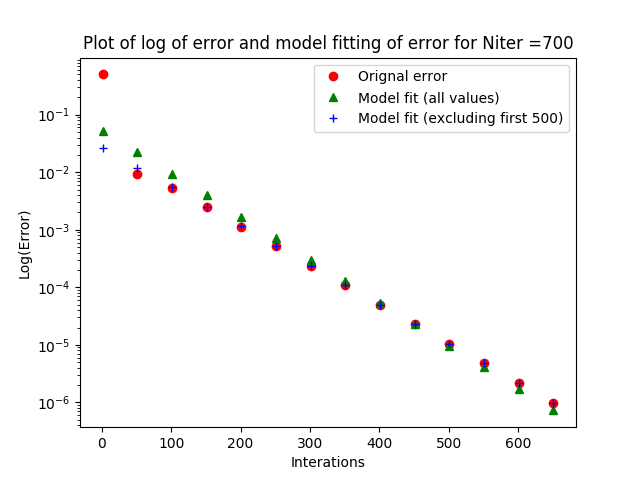
\includegraphics{Figure_1-8.png}
\end{figure}
Clearly from the plots (See Figure 8 and 9) it is clear that removing first 500 iteration gives a better fit. The difference is ore clear with less iterations at higher valve all seem to converge.
\begin{lstlisting}[language=Python]
#fitting the obtained coefficients with the orignsl error.
c = np.ones(Niter)
xiter = np.arange(1,Niter+1)
fit_1_v = c*fit_1[0] + (xiter)*fit_1[1]
fit_2_v = c*fit_2[0] + (xiter)*fit_2[1]

plt.plot(xiter[::50],np.log(errors)[::50],"ro")
plt.plot(xiter[::50],fit_1_v[::50],"g^")
plt.plot(xiter[::50],fit_2_v[::50],"b+")
plt.xlabel("Interations")
plt.ylabel("Log(Error)")
plt.title("Plot of log of error and model fitting of error for Niter ="+str(Niter))
plt.legend(["Orignal error","Model fit (all values)","Model fit (excluding first 500)"])
plt.show()
\end{lstlisting}
$$ Error = \sum_{k=Niter+1}^{\infty} error_{k} $$
$$ Error \textless \sum_{k=Niter+1}^{\infty} Ae^{Bk} $$
$$Error \approx \int_{Niter+0.5}^{\infty} Ae^{Bk} dk  $$
$$Error \approx \frac{-A}{B}exp(B(Niter+0.5)) $$

From the above result if we calculate Error by substituting values we obtained.Maximum error from the result and and the last per iteration change in phi (last value of error) do not match.
Since error falls as Ae$^{Bk}$ , $\frac{1}{B}$ is the half life. Error obtained times halflife will give us correct value which seems to match in the output.
\begin{lstlisting}[language=Python]
#for 700 iterations
A   0.0241262089052
B  -0.014197697826
Max error = -A/B exp(B(Niter + 1)) 8.08942957309e-05
Max Error times half life -1.14851276663e-06
Error in last step 1.16492469504e-06
\end{lstlisting}
\begin{lstlisting}[language=Python]
#for 1500 iterrations
A   0.0241282489
B  -0.0141978380383
Max error = -A/B exp(B(Niter + 1)) 9.44220600578e-10
Max Error times half life -1.34058911594e-11
Error in last step 1.35974564941e-11

\end{lstlisting}
\section{Current Heating }
From Current value from the previous part we can calculate temperature at all points to know the heating effect. It can be done from the equation below.
$$ \nabla . (k \nabla T) = -\frac{1}{\sigma}\mid{J}\mid^{2} $$
Solving this similarly as we did for potential
$$ \frac{dT}{dx}_{(x_{i},y_{i})} = \frac{T(x_{i+1/2},y_{j})-T(x_{i-1/2},y_{j})}{\Delta x} $$
and
$$ \frac{d^{2}T}{dx^{2}}_{(x_{i},y_{i})} = \frac{T(x_{i+1},y_{j})-2T(x_{i},y_{j})+T(x_{i-1},y_{j})}{\Delta x} $$
From the above equation we can obtain the steady state temperature at any point as
$$T_{i,j} = \frac{T_{i-1,j}+T_{i,j-1}+T_{i,j+1}+T_{i+1,j} +\frac{\Delta x^{2}}{k\sigma}\mid J_{i,j}^{2} \mid}{4}$$
With the given initial conditions given , wire and the grounded side at 300. And $\frac{dT}{dn} = 0$ (change in T along normal component at all other sides is 0). See Figure 8. 
\begin{lstlisting}[language=Python]
dx = Nx/24
temp = np.zeros((Nx,Ny))
temp[ii] = 300 
temp[-1,:] = 300
for k in range(Niter):
	#specifying initial conditions
	temp[1:-1,1:-1] = 0.25*(temp[1:-1,0:-2]+temp[1:-1,2:]+temp[0:-2,1:-1]+temp[2:,1:-1]+(dx**2/(sigma*kappa))*((Jx[1:-1,1:-1]**2+Jy[1:-1,1:-1]**2))) #updating potential as mean of its neighbors
	temp[1:-1,0] = temp[1:-1,1] # Boundary Conditions
	temp[0,:] = temp[1,:]
	temp[1:-1,-1] = temp[1:-1,-2]
	temp[-1,:] = 300
	temp[ii] = 300	

fig1 = plt.figure(1)
ax = p3.Axes3D(fig1)
plt.title('The 3-D surface plot of temperature')
surf = ax.plot_surface(-Y,-X,temp.T,rstride = 1,cstride = 1, cmap = plt.cm.jet)
plt.show()
\end{lstlisting}
\begin{figure}
\caption{}
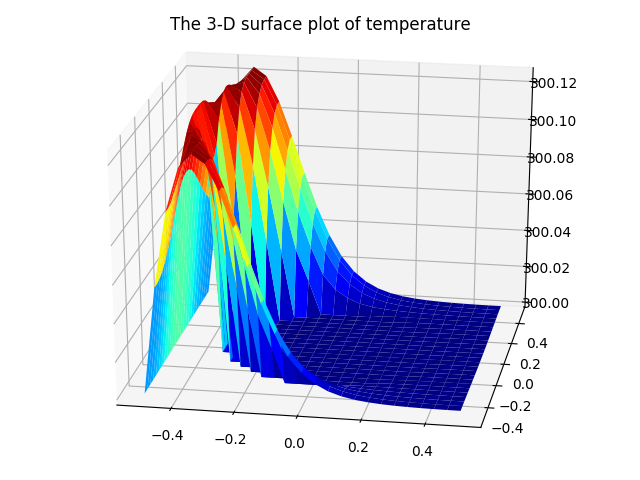
\includegraphics{Figure_1-9.png}
\end{figure}
\subsection{Explanation for Temperature plot of surface}
As seen from Figure 8 . The resistor heats up more at the point where current flowing is more. The upper half of the plate remain at 300 as no current flows there.
\end{document}

